\chapter{Active Directory Pentesting: Objectives, Methodology, and Testing Approaches}

\abstract{Active Directory (AD) is at the core of many organizations' IT infrastructure, responsible for authentication, authorization, and access to critical resources. This chapter outlines the objectives, methodology, and phases of an AD penetration test, covering both black-box (unauthenticated) and grey-box (authenticated) scenarios. Practical use cases, common vulnerabilities, and misconfigurations are discussed to highlight how attackers operate and how defenders can prepare.}
\label{ch:ad-pentesting}

\section{Introduction}
Active Directory (AD) underpins identity and access management for the majority of enterprise environments. By centralizing users, computers, and policies, AD provides efficiency but also introduces a large attack surface. A single misconfiguration or unpatched vulnerability can enable an attacker to compromise the entire domain.

\warningbox{\lipsum[4]}



Because of this, \textbf{Active Directory penetration testing (AD pentesting)} has become a critical defensive practice. AD pentesting simulates real-world attacks to identify exploitable weaknesses, misconfigurations, and privilege escalation paths before adversaries can abuse them. This chapter explains the objectives, scope, and structured methodology of AD pentesting, highlighting the differences between black-box and grey-box testing.

\begin{figure}[htbp]
  \justifying
 % \includegraphics[width=0.8\textwidth]{images/active-directory-pentesting.png}
  \caption{Active Directory Pentesting Overview}
  \label{fig:ad-pentesting-overview}
\end{figure}

\section{What is Active Directory Pentesting?}
AD pentesting is a specialized security assessment targeting the AD environment itself. Unlike general network penetration testing, AD pentesting focuses on the infrastructure that governs authentication, authorization, and trust relationships.

\begin{itemize}
  \item \textbf{Domain Controllers:} The servers that enforce policies, authenticate users, and replicate directory data.
  \item \textbf{Users and Groups:} Accounts, memberships, and privilege assignments.
  \item \textbf{Security Policies:} Password policies, Kerberos configurations, and access controls.
  \item \textbf{Network Services:} LDAP, SMB, Kerberos, DNS, and hybrid cloud connectors (e.g., Azure AD).
\end{itemize}

The goal is not merely to scan for vulnerabilities but to demonstrate realistic attack paths that could compromise confidentiality, integrity, or availability of the domain.

\section{Objectives of AD Pentesting}
The primary objectives are:
\begin{enumerate}
  \item Identify weaknesses in domain controllers, accounts, and policies.
  \item Simulate real attack vectors such as credential theft, relay attacks, and privilege escalation.
  \item Evaluate the resilience of monitoring and logging controls.
  \item Provide actionable recommendations to harden the AD environment.
\end{enumerate}

A successful pentest report does not only list vulnerabilities but shows how an attacker could pivot from a single foothold to complete domain compromise.

\section{Scope Definition}
The scope of an AD pentest is tailored to organizational needs. It may include:
\begin{itemize}
  \item Full enterprise domains and forests.
  \item Specific subnets, OUs, or trust boundaries.
  \item Critical components such as domain controllers, PKI (AD CS), and privileged groups.
  \item Externally exposed interfaces (VPN, RDP gateways, hybrid cloud connectors).
\end{itemize}

Clear scoping ensures tests remain focused and risk-controlled, while also aligning with business objectives.

\section{Methodology}
AD pentesting follows a structured methodology adapted from standard penetration testing frameworks but with AD-specific nuances:

\begin{enumerate}
  \item \textbf{Planning and Scoping:} Define rules of engagement, target systems, and objectives.
  \item \textbf{Reconnaissance:} Collect information on domains, accounts, and topology (human + technical recon).
  \item \textbf{Enumeration:} Use tools (e.g., BloodHound, LDAP queries) to map users, groups, ACLs, and trust paths.
  \item \textbf{Vulnerability Assessment:} Identify CVEs, weak configurations, and policy gaps.
  \item \textbf{Exploitation:} Attempt privilege escalation and lateral movement through realistic attack paths.
  \item \textbf{Post-Exploitation:} Demonstrate impact (e.g., domain admin compromise, data exfiltration).
  \item \textbf{Reporting and Remediation:} Deliver findings with actionable mitigations.
\end{enumerate}

\begin{figure}[htbp]
  \justifying
  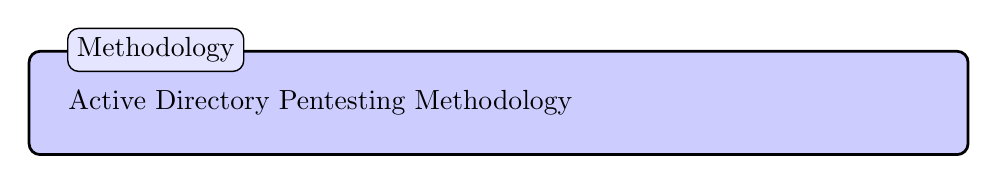
\begin{tikzpicture}
    \node[anchor=text,text width=\columnwidth-1.2cm, draw, rounded corners,
          line width=1pt, fill=blue!20, inner sep=5mm] (big) {Active Directory Pentesting Methodology};
    \node[draw, rounded corners, line width=.5pt, fill=blue!10, anchor=west,
          xshift=5mm] (small) at (big.north west) {Methodology};
  \end{tikzpicture}
  \caption{Active Directory Pentesting Methodology}
  \label{fig:ad-pentesting-methodology}
\end{figure}

\section{Pentesting Phases}
\subsection{Reconnaissance}
Human reconnaissance targets people (admins, IT staff) via OSINT and social engineering opportunities, while technical reconnaissance focuses on network enumeration, AD schema discovery, and service fingerprinting.

\subsection{Exploitation}
Two testing models are common:
\begin{itemize}
  \item \textbf{Black Box (Unauthenticated):} Simulates an external attacker with no credentials. Relies heavily on scanning, exploiting CVEs (e.g., Zerologon, PetitPotam), and abusing default protocols (e.g., LLMNR/NBT-NS poisoning).
  \item \textbf{Grey Box (Authenticated):} Simulates an insider or compromised user account. Enables deeper enumeration (BloodHound, LDAP queries) and exploitation of misconfigurations (weak ACLs, DACL abuse, AD CS misconfigurations).
\end{itemize}

\section{Common Attack Scenarios}
\begin{itemize}
  \item \textbf{Credential Abuse:} Kerberoasting, ASREPRoasting, Pass-the-Hash, and Pass-the-Ticket attacks.
  \item \textbf{Network Abuse:} LLMNR/NBT-NS/mDNS spoofing, DHCPv6 poisoning.
  \item \textbf{Privilege Escalation:} Exploiting misconfigured ACLs, trusts, or Group Policy Objects.
  \item \textbf{Domain Controller Exploits:} Zerologon (CVE-2020-1472), PrintNightmare, SMBGhost, EternalBlue.
  \item \textbf{Certificate Abuse:} Exploiting Active Directory Certificate Services (AD CS) for persistence or domain escalation.
\end{itemize}

\section{Conclusion}
Active Directory pentesting is a critical discipline that blends offensive security with defensive insights. By simulating realistic attack paths—whether from an outsider’s perspective (black box) or an insider’s (grey box)—organizations can uncover dangerous weaknesses before adversaries do. A well-executed AD pentest provides not just vulnerabilities, but a roadmap for strengthening resilience against the attacks most likely to succeed in the real world.
